\chapter*{Version and reproducibility}\label{book-reproducibility}
\addcontentsline{toc}{chapter}{Version and reproducibility}

\section*{The code this edition teaches}

This edition uses published Bijou 7.2.0 and the companion's \texttt{book-v2} tag. Clone the exact edition, run \texttt{npm ci}, then follow the five independent build stages. The original \texttt{book-v1} remains available. Historical source records describe their original versions and do not change the teaching dependency manifest.

\begin{center}
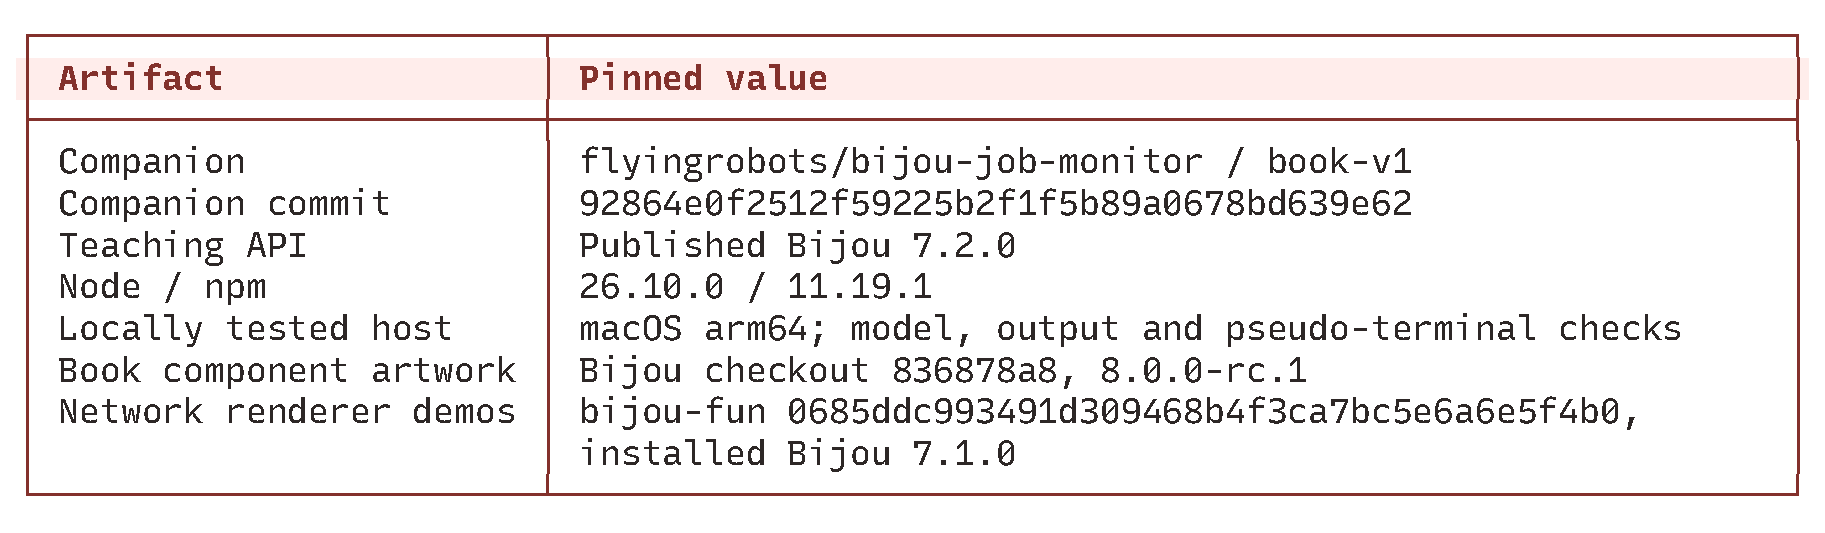
\includegraphics[width=\linewidth]{figures/tables/edition-versions-g1-1.pdf}
\par\smallskip{\scriptsize\color{BookMuted}Rows 1–7. Actual Bijou table component.}
\end{center}


\subsection*{The tested boundary}

The companion typechecks and passes 44 tests across eight files. A clean candidate install also ran every stage with the finished source hidden. Four actual source diffs were verified. Six local pseudo-terminal cases exercised keyboard input, resizing, quit and SIGTERM for stages 03, 04 and 05 and verified restoration of canonical-input and echo flags. Those cases observe output and lifecycle; deterministic App and model tests establish input semantics. The recorded host was macOS arm64. Hosted CI status belongs to its recorded run at the pinned commit.

\subsection*{Human observations remain separate}

The unfamiliar-reader walkthrough is prepared and has not been conducted. A participant session is planned; no observations have been recorded. Its protocol and blank form are included in the companion and summarized in the book appendix. No screen-reader usability study or broad emulator matrix is claimed. The accessible CLI prints a fixture and exits; an interactive screen-reader workflow is not implemented.

\subsection*{Build stages and inspections}

Use \texttt{npm run stage -- 01} through \texttt{05}, \texttt{npm run stage:check -- 01}, and \texttt{npm run stage:diff -- 01 02}. Each stage owns its source modules and shares only the root dependency lock. The older \texttt{checkpoint} commands inspect the completed implementation. The workshops distinguish those two routes explicitly.

Report corrections at \url{https://github.com/flyingrobots/bijou-job-monitor/issues}, including the edition commit, stage or workshop, command and environment. The fonts used for printed specimens are publication choices, not assumptions about the reader's terminal.
